% !TEX program = lualatex
\documentclass[12pt,a4paper]{article}
\usepackage{amsmath,amssymb,amsthm}
\usepackage{geometry}
\geometry{margin=2.5cm}
\usepackage{hyperref}
\hypersetup{colorlinks=true,linkcolor=blue,citecolor=blue,urlcolor=blue}
\usepackage{booktabs}
\usepackage{lmodern}
\usepackage[T1]{fontenc}
\usepackage{graphicx}

\title{Realization of Perfectly Elastic Collision in the Delay Circuit Model}
\author{Noriaki Kihara\\
WF System Co., Ltd.\\
Osaka University, School of Engineering Science (graduated)}
\date{April 2026\quad Research Note\\[4pt]
DOI: \href{https://doi.org/10.5281/zenodo.19534353}{10.5281/zenodo.19534353}}

\begin{document}

\maketitle

\begin{abstract}
We extend class $B$ (transverse wave) defined in the previous paper~\cite{ref3} to define class $E$, which holds position information and displacement. After constructing a non-interacting model in which two instances of class $E$ propagate in opposite directions, we define class $F$, which adds a collision radius $r$ per instance and the perfectly elastic collision formula to the operation function $*$. By treating $w_{\max}$ as an analogue of mass, a perfectly elastic collision satisfying conservation of momentum and energy is realized. The definitions of the delay circuit $F_D$ and the NOT operation circuit are not changed.
\end{abstract}

\section{Introduction}

In the previous paper~\cite{ref1}, oscillation and propagation patterns were constructed using the delay circuit $F_D$ and the NOT operation circuit. In the previous paper~\cite{ref2}, the framework of superclasses, meta-information, and the operation function $*$ was introduced. In the previous paper~\cite{ref3}, class $B$ was used to realize a sine wave (transverse wave).

In this paper, we define class $E$ as an extension of class $B$, and treat the case in which two instances propagate in opposite directions on the same open rope model. We first construct a model without interaction (passing through), and then construct a model that realizes a perfectly elastic collision.

\section{Preparation: Summary of Definitions from Previous Papers}

This paper presupposes the delay circuit $F_D$ and the NOT operation circuit from the previous paper~\cite{ref1}, the superclass, meta-information, and operation function $*$ from the previous paper~\cite{ref2}, and class $B$ (transverse wave) from the previous paper~\cite{ref3}. For details of these definitions, refer to the respective previous papers.

\section{Definition of Class $E$}

\subsection{Information and Meta-information of Class $E$}

We extend class $B$ (\cite{ref3}, \S3.4) and define class $E$ with position information as follows.

\paragraph{Information of class $E$:}

\begin{itemize}
  \item $i$: scalar value (input value; identical to class $B$)
  \item $w$: real value (amplitude; for output; identical to class $B$)
  \item $x_0$: initial position (integer value)
  \item $x$: current position (real value)
  \item $dx$: displacement (integer value; position change per step)
\end{itemize}

\paragraph{Meta-information:}

\begin{itemize}
  \item $n$: counter (number of delays)
  \item $m$: number of delays corresponding to one wavelength
  \item $w_{\max}$: maximum amplitude (positive real value)
  \item color: attribute for identification
\end{itemize}

\subsection{Operation Function $*$}

\begin{equation}
  x = n \cdot dx + x_0
\end{equation}

\begin{equation}
  w = w_{\max} \cdot \sin\!\left(\frac{n}{m} \cdot 360°\right)
\end{equation}

Each time $F_D$ is passed, $n$ is incremented and the position $x$ and amplitude $w$ are updated.

\section{Non-interacting Model (Passing Through)}

\subsection{Definition of Two Instances}

We define two instances of class $E$.

\paragraph{$E_1$ (red):}

\begin{table}[h]
  \centering
  \begin{tabular}{@{}ll@{}}
    \toprule
    Information / Meta-information & Value \\
    \midrule
    $x_0$       & 0   \\
    $x$         & 0   \\
    $dx$        & $+1$ \\
    $m$         & 12  \\
    $w_{\max}$  & 2   \\
    color       & red \\
    \bottomrule
  \end{tabular}
  \caption{Initial conditions of $E_1$ (red)}
\end{table}

\paragraph{$E_2$ (blue):}

\begin{table}[h]
  \centering
  \begin{tabular}{@{}ll@{}}
    \toprule
    Information / Meta-information & Value \\
    \midrule
    $x_0$       & 24   \\
    $x$         & 24   \\
    $dx$        & $-1$ \\
    $m$         & 12   \\
    $w_{\max}$  & 1    \\
    color       & blue \\
    \bottomrule
  \end{tabular}
  \caption{Initial conditions of $E_2$ (blue)}
\end{table}

\subsection{Sequence of Passing Through}

$E_1$ and $E_2$ execute the operation $*$ independently and do not affect each other. The position at each step is shown below.

\begin{table}[h]
  \centering
  \begin{tabular}{@{}ccc@{}}
    \toprule
    $n$ & $x$ of $E_1$ & $x$ of $E_2$ \\
    \midrule
    0         & 0          & 24         \\
    1         & 1          & 23         \\
    2         & 2          & 22         \\
    $\vdots$  & $\vdots$   & $\vdots$   \\
    12        & 12         & 12         \\
    $\vdots$  & $\vdots$   & $\vdots$   \\
    24        & 24         & 0          \\
    \bottomrule
  \end{tabular}
  \caption{Positions of $E_1$ and $E_2$ at each step (non-interacting model)}
\end{table}

At $n = 12$, $E_1$ and $E_2$ reach the same position $x = 12$, but since there is no interaction they pass through each other, and at $n = 24$ each reaches the initial position of the other.

\subsection{Visualization of Passing Through}

The spacetime diagram below shows the trajectories of $E_1$ (red) and $E_2$ (blue). The horizontal axis is position $x$ and the vertical axis is the number of delays $n$ (progressing from top to bottom). The size of each point corresponds to the amplitude $|w|$; dark color represents $w > 0$ and light color represents $w < 0$.

\begin{figure}[h]
  \centering
  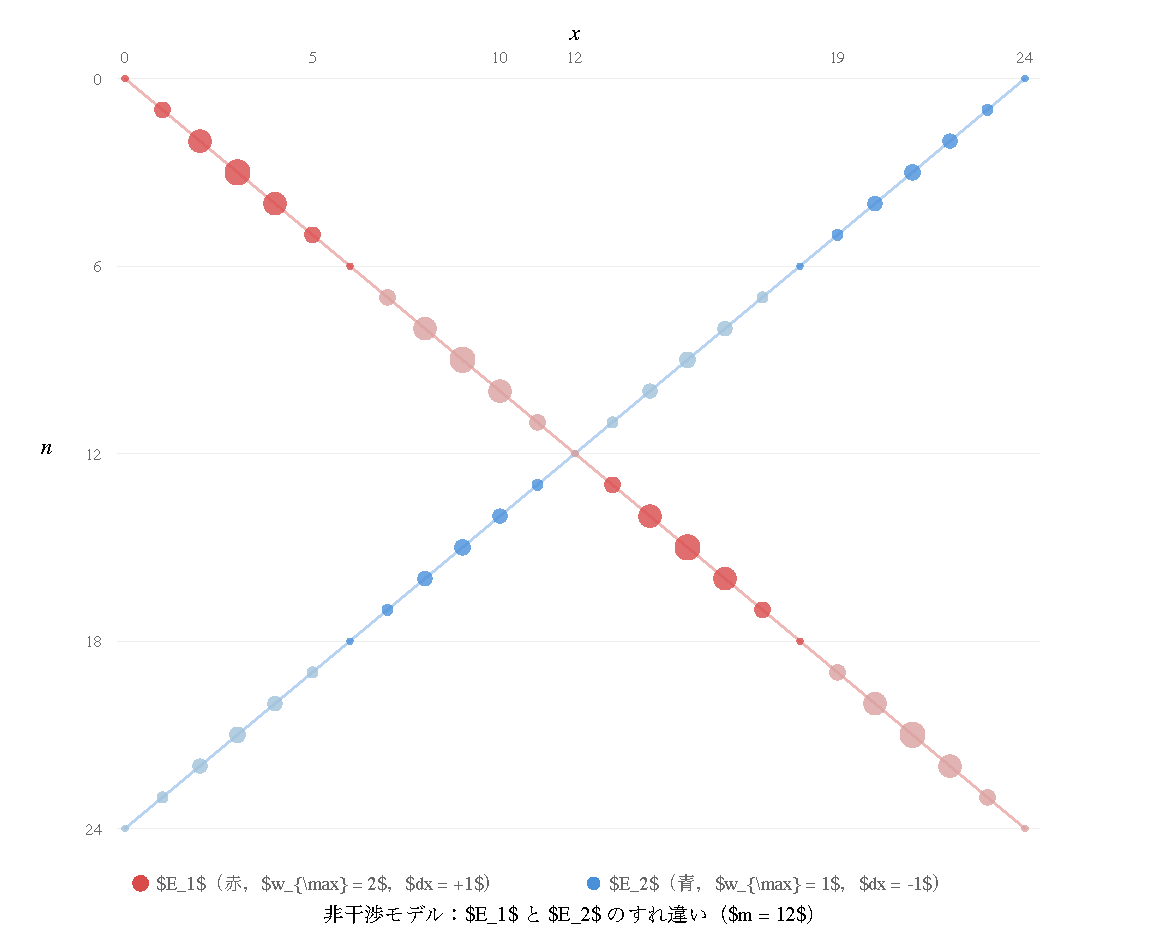
\includegraphics[width=0.8\linewidth]{fig9_pass_through.pdf}
  \caption{Non-interacting model --- passing through of $E_1$ and $E_2$ ($m = 12$). At $n = 12$, both pass through the same position $x = 12$, but since there is no interaction they continue straight ahead without any effect on each other.}
  \label{fig:pass_through}
\end{figure}

\section{Model of Perfectly Elastic Collision}

\subsection{Definition of Class $F$}

We extend class $E$ (\S3) to define class $F$, which has collision functionality. The information and meta-information of class $F$ are identical to those of class $E$, with the following meta-information added:

\begin{itemize}
  \item $r$: collision radius (a real number with $r > 0$; each instance may have a different value)
\end{itemize}

\paragraph{Collision Detection.}

For two instances $F_1$ (collision radius $r_1$) and $F_2$ (collision radius $r_2$), a collision is detected when the following condition is satisfied:

\begin{equation}
  (x_1 - x_2)^2 < \max(r_1^2,\; r_2^2)
\end{equation}

\paragraph{Update of $dx$ at Collision.}

When a collision occurs, $dx$ is updated using the one-dimensional perfectly elastic collision formula, treating $w_{\max}$ as an analogue of mass:

\begin{equation}
  dx_1^{\text{new}} = \frac{(w_{\max,1} - w_{\max,2}) \cdot dx_1 + 2\, w_{\max,2} \cdot dx_2}{w_{\max,1} + w_{\max,2}}
\end{equation}

\begin{equation}
  dx_2^{\text{new}} = \frac{(w_{\max,2} - w_{\max,1}) \cdot dx_2 + 2\, w_{\max,1} \cdot dx_1}{w_{\max,1} + w_{\max,2}}
\end{equation}

This update maintains the following two conserved quantities:

\begin{itemize}
  \item \textbf{Analogue of momentum}: $Q = w_{\max,1} \cdot dx_1 + w_{\max,2} \cdot dx_2$
  \item \textbf{Analogue of energy}: $K = w_{\max,1} \cdot dx_1^2 + w_{\max,2} \cdot dx_2^2$
\end{itemize}

\subsection{Sequence of Collision}

Using the same initial conditions as \S4.1, and setting $r_1 = r_2 = 1$ for simplicity.

\paragraph{Before collision ($n < 12$):}

The trajectories are identical to those of $E_1$ and $E_2$ (see \S4.2).

\paragraph{Collision at $n = 12$:}

From $(x_1 - x_2)^2 < \max(r_1^2, r_2^2)$, a collision is detected. $dx$ is updated:

\begin{equation}
  dx_1^{\text{new}} = \frac{(2-1)(1) + 2(1)(-1)}{2+1} = \frac{-1}{3} = -\frac{1}{3}
\end{equation}

\begin{equation}
  dx_2^{\text{new}} = \frac{(1-2)(-1) + 2(2)(1)}{2+1} = \frac{5}{3}
\end{equation}

\paragraph{Verification:}

\begin{equation}
  Q^{\text{new}} = 2 \cdot (-1/3) + 1 \cdot (5/3) = -2/3 + 5/3 = 1 = Q \quad \checkmark
\end{equation}

\begin{equation}
  K^{\text{new}} = 2 \cdot (1/9) + 1 \cdot (25/9) = 27/9 = 3 = K \quad \checkmark
\end{equation}

\paragraph{After collision ($n > 12$):}

\begin{table}[h]
  \centering
  \begin{tabular}{@{}ccc@{}}
    \toprule
    $n$ & $x$ of $F_1$ & $x$ of $F_2$ \\
    \midrule
    12 & 12.00 & 12.00 \\
    13 & 11.67 & 13.67 \\
    14 & 11.33 & 15.33 \\
    15 & 11.00 & 17.00 \\
    18 & 10.00 & 22.00 \\
    21 &  9.00 & 27.00 \\
    24 &  8.00 & 32.00 \\
    \bottomrule
  \end{tabular}
  \caption{Positions of $F_1$ and $F_2$ after the collision}
\end{table}

The heavier $F_1$ with $w_{\max} = 2$ slowly returns in the reverse direction ($dx = -1/3$), while the lighter $F_2$ with $w_{\max} = 1$ is knocked away at high velocity ($dx = 5/3$).

\subsection{Visualization of Collision}

The spacetime diagram below shows the trajectories of $F_1$ (red) and $F_2$ (blue). At the collision point at $n = 12$ (dashed circle), both trajectories bend. The heavier $F_1$ slowly returns to the left after the collision, while the lighter $F_2$ is knocked away to the right at high velocity.

\begin{figure}[h]
  \centering
  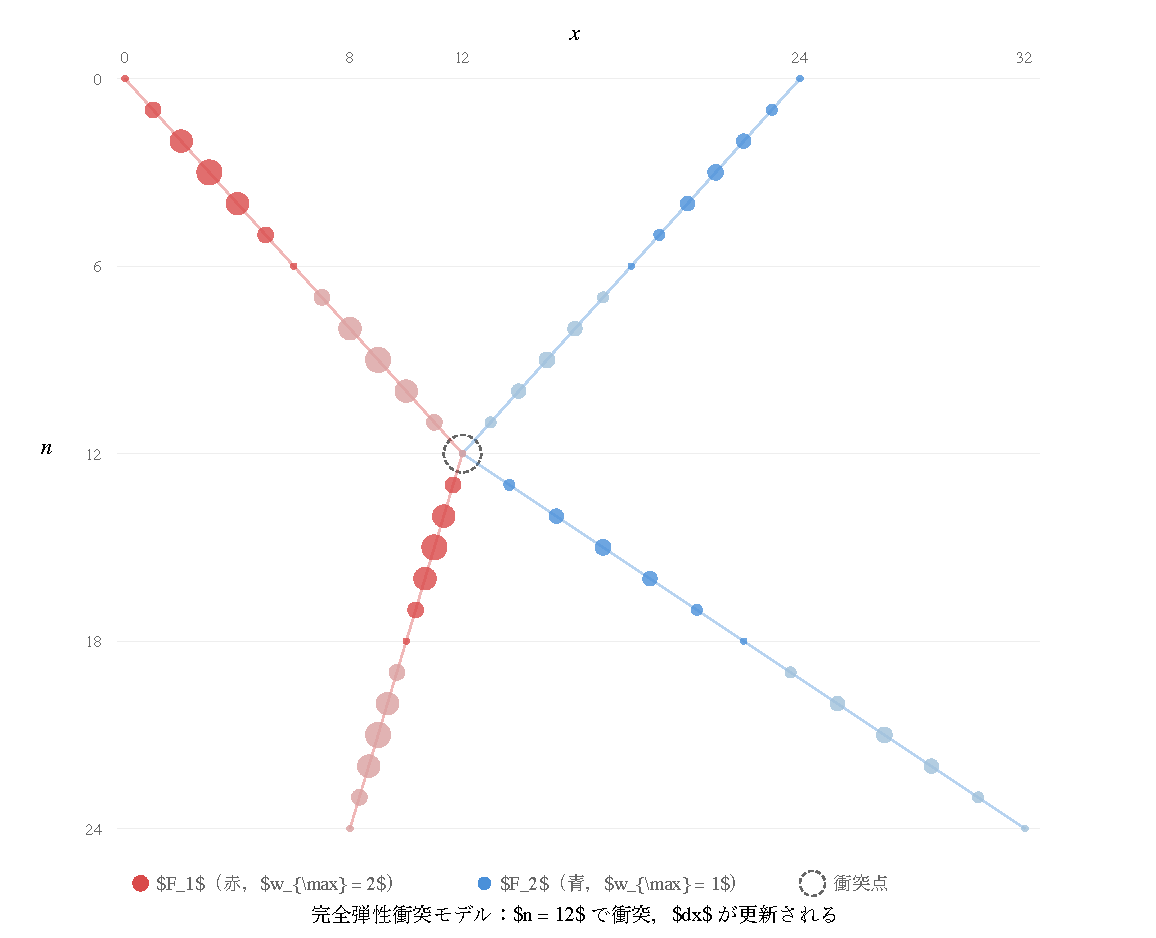
\includegraphics[width=0.8\linewidth]{fig10_elastic_collision.pdf}
  \caption{Perfectly elastic collision model --- collision at $n = 12$, $dx$ is updated. Comparing with Figure~\ref{fig:pass_through} (non-interacting model), the trajectories before the collision ($n < 12$) are identical, but after the collision ($n > 12$) the slopes of the trajectories change to reflect the mass ratio (the ratio of $w_{\max}$).}
  \label{fig:elastic_collision}
\end{figure}

\section{Conclusion}

We extended class $E$ (\S3) to define instances with position information and displacement. For the case in which two instances propagate in opposite directions on the same space, we first constructed a non-interacting model (\S4, passing through), and then realized a perfectly elastic collision by adding a collision radius $r$ and the perfectly elastic collision formula to the operation function $*$ via class $F$ (\S5).

In either case, the definitions of the delay circuit $F_D$ and the NOT operation circuit are not changed. The presence or absence of interaction is expressed solely as a difference in the definition of the operation function~$*$.

\begin{thebibliography}{9}

\bibitem{ref1}
Noriaki Kihara,
``Information-Theoretic Organization of Information Transmission,''
Research Note, April 2026.

\bibitem{ref2}
Noriaki Kihara,
``Organization of Symmetries Inherent in the Delay Circuit Model,''
Research Note, April 2026.

\bibitem{ref3}
Noriaki Kihara,
``Realization of Simple Harmonic Oscillation and Sinusoidal Waves in the Delay Circuit Model,''
Research Note, April 2026.

\end{thebibliography}

\end{document}
